\documentclass[a4paper,10pt]{article}
\usepackage[utf8]{inputenc}
\usepackage{enumerate}
\usepackage{amsmath}
\usepackage{graphicx}
\usepackage{listings}
\usepackage{float}
\usepackage[caption = false]{subfig}
\usepackage[parfill]{parskip}
\usepackage{url}

\title{Project 3: Stellar Convection}
\author{Christer Dreierstad\footnote{I have been working together with Hans Erlend Bakken Glad.}}
\date{25.05.2018}

\begin{document}
\maketitle
\section{Introduction}
I have not been successful in creating a code that produces anything that makes sense beyond the initial conditions, so I will discuss the process, what I have attempted to solve and what I have achieved. There are small footnotes with comments regarding uncertainties in the method.

\section{Model}
Creating a box that has $x=y=0$ at the lowest left corner, so that y is positive upwards and x positive to the right. We consider the amount of particles $N = n_x\times n_y$, where $n_x$ and $n_y$ are the particles stacked in x and y direction respectively. Since we wish to calculate over a distance of $12$ Mm in the x-direction, and $4$ Mm in the y-direction, we choose $dx = nx/12\times 10^6$ and $dy = ny/4 \times 10^6$. Since the box is small compared to the entirety of the star, we consider the gravitation to be constant, given by the mass and the radius of the sun. When calculating the various values of the star, we assume the density, pressure and temperature to be constant for all x for each y value, i.e. we assume them to be constant for each layer y in the box.

\section{Analytics}
\subsection{Initial conditions}
At the top of the box, being the surface of the star, we set the initial condition for temperature and pressure to be the same as the average temperature and pressure of the photosphere of the star, 5778 K and $1.8 \cdot 10^8$ Pa respectively. Since the velocities at time $t = 0$ is zero for all the particles the fluid is in hydrostatic equilibrium. The equation of conservation of energy for $\rho u_y$ is given as
%
\begin{align}\label{eq:dpuy_dt}
\frac{\partial \rho u_y}{\partial t} = -\frac{\partial \rho u_y u_x}{\partial x} - \frac{\partial \rho u_y u_y}{\partial y} - \frac{\partial}{\partial y} P - g\rho,
\end{align}
%
where $-g\rho$ is the source of gravitation. Initially all velocities are zero, and there is no change in momentum, so all the terms above except the last to on the right are zero. From this we then have a gradient for the pressure in y-direction, given by the last two terms in the equation above:
\begin{align}\label{eq:dP_dy}
\frac{\partial P}{\partial y} = -g\rho,
\end{align}
%
which we know as hydrostatic equilibrium. We choose the double logarithmic gradient $\nabla = \partial \ln T/\partial \ln P = 0.5$. From this we find a gradient for the temperature:
%
\begin{align*}
0.5 = \nabla = \frac{\partial \ln T}{\partial \ln P} = \frac{P}{T}\frac{\partial T}{\partial P} = \frac{P}{T}\frac{\partial T}{\partial y}\frac{\partial y}{\partial P},
\end{align*}
%
where $dP/dy$ is the gradient we found above. We then solve the equation for the vertical gradient of the temperature and get:
%
\begin{align}\label{eq:dT_dy}
\frac{\partial T}{\partial y} = \nabla \frac{T}{P}\frac{\partial P}{\partial y} = 0.5\frac{T}{P}\frac{\partial P}{\partial y}.
\end{align}
With the initial values for pressure and temperature being that of the photosphere of the sun, we can find the initial conditions for density and energy by the equation of state and (F.13) respectively. So to calculate the initial condition for the density and energy we have the equation of state solved for the density
%
\begin{align}\label{eq:eos}
\rho = P\frac{\mu m_u  }{kT} = \frac{e}{(\gamma - 1)}\frac{\mu m_u}{kT}
\end{align}
%
and the internal energy equation
%
\begin{align}
e = \frac{\rho k T}{\mu m_u}(\gamma - 1),
\end{align}
 where $\mu$ is the chemical potential, which we set equal to $0.61$ since we assume an ideal gas, $m_u$ is the unified atomic mass, $\gamma = c_P/c_V = (5k/2\mu m_u)/(3k/2\mu m_u) = 5/3$, and $k$ is Boltzmann's constant. 

\subsection{Boundary conditions}
Since we are considering a constant number of particles and we do not want to keep refilling the box during the simulation, we set the horizontal boundary to be circular. With a circular horizontal boundary we consider a change in the fluid that exits the box at one side, to appear on the other side. This is a good approximation, considering that particles in the fluid moves constantly, so on average one would see this kind of behavior. We cannot make such an approximation for the vertical boundary, as this would mean we let particles escape the box, which again means  we let particles escape the star we simulate. 

By setting the velocities to be zero at the vertical boundary, we can see by equation \eqref{eq:dpuy_dt} that we have hydrostatic equilibrium at the vertical boundaries, and therefore no particles will escape the star. This also means we have a gradient for the pressure at the boundaries, given by equation \eqref{eq:dT_dy}. Also, since we are setting the velocities at the vertical boundary to be zero, we also make sure that there is no momentum passing out of the star, i,e. the gradient of the momentum $\partial \rho u_i/\partial x_k = 0$ at the boundary. Further we set the vertical gradient of the horizontal component of the velocity to be 0, meaning that $\partial u_x/\partial y = 0$. To make the fluid unstable, we force a temperature difference in the fluid, such that the temperature on the top of the box is $0.9T_0$, and $1.1T_0$ at the bottom, where $T_0$ is the average temperature of the sun at photosphere.

The boundary condition for energy was found by using the internal energy equation (F.13) and inserting the boundary condition for temperature discussed above. To find the boundary condition for density we use the equation of state inserting the boundary condition for the energy and temperature. 

\subsection{Hydrodynamic equations}
To simulate the movement of the fluid we need the hydrodynamic equations. First we consider the continuity equation, without sources or sinks, 
%
\begin{align}\label{eq:cons_mass}
\frac{\partial \rho}{\partial t} &= -\nabla \cdot \left(\rho u_i\right) = -\left(\rho \nabla \cdot u_i + u_i\nabla \rho\right) \nonumber \\
&= -\left(\rho \frac{\partial u_i}{\partial x_k} + u_i \frac{\partial \rho}{\partial x_k}\right),
\end{align}
%
where $\rho$ is the density, i denotes the direction of the variable, in this case $u_i$ being the bulk velocity in directions x and y. Solving the equation for both directions we get:
%
\begin{align}
\frac{\partial \rho}{\partial t} &= -\rho\frac{\partial u_x}{\partial x} - \rho \frac{\partial u_y}{\partial y} - u_x\frac{\partial \rho}{\partial x} - u_x\frac{\partial \rho}{\partial y} \nonumber -  \rho\frac{\partial u_y}{\partial x} - \rho \frac{\partial u_y}{\partial y} - u_y \frac{\partial \rho}{\partial x} - u_y \frac{\partial \rho}{\partial y} \nonumber \\
&= -\rho\left[\frac{\partial u_x}{\partial x} + \frac{\partial u_x}{\partial y} + \frac{\partial u_y}{\partial x} + \frac{\partial u_y}{\partial y}\right] - \left(u_x + u_y\right)\left[2\frac{\partial \rho}{\partial x} + 2\frac{\partial \rho}{\partial y}\right].
\end{align}



The equation of motion, 
%
\begin{align}\label{eq:cons_motion}
\frac{\partial \rho u_i}{\partial t} &= -\nabla \cdot \left(\rho u_i u_k\right) - \nabla P\delta_{ik} + F \nonumber \\
&= -\left( u_k \frac{\partial \rho u_i}{\partial x_k} + \rho u_i \frac{\partial u_k}{\partial x_k} \right) -\frac{\partial P\delta_{ik}}{\partial x_k} + F
\end{align}
%
where $P$ is the thermal pressure, multiplied by the delta function. The above equation has the viscous stress tensor set to zero, as we will not consider viscosity in this paper. The pressure is constant in concentric layers of y values, therefore the pressure gradient in x is zero. F is the term for gravitation acting on the fluid, which is $g\rho$ when $x_k = y$. When solving this equation, we use the product rule for the first two terms on the right, an example of how this is done for $\rho u_y$ follows:
%
\begin{align*}
\frac{\partial \rho u_y}{\partial t} &= -\frac{\partial}{\partial x_k}\left(\rho u_y u_k\right) \nonumber \\
 &= -\left[\frac{\partial}{\partial x}\left(\rho u_y u_x\right) + \frac{\partial }{\partial y}\left(\rho u_y u_y\right)\right] \nonumber \\
 &= -\left[\rho u_y \frac{\partial u_x}{\partial x} + u_x\frac{\partial \rho u_y}{\partial x} + \rho u_y \frac{\partial u_y}{\partial y} + u_y \frac{\partial \rho u_y}{\partial y}\right] \nonumber \\
 &= -\rho u_y\left(\frac{\rho u_x}{\partial x} + \frac{\partial u_y}{\partial y}\right) - u_x \frac{\partial \rho u_y}{\partial x} - u_y \frac{\partial \rho u_y}{\partial y}.
\end{align*}
%
The same approach goes for $u_x$. Lastly the equation of energy, without any sources or sinks
%
\begin{align}\label{eq:cons_energy}
\frac{\partial e}{\partial t} &= -\nabla \cdot \left(eu_i\right) - P\nabla u_i \nonumber \\
&= -\frac{\partial eu_i}{\partial x_k} - P\frac{\partial u_i}{x_k}
\end{align}
where e is the internal energy per unit mass. Solving this equation for both directions of bulk velocity and all directions we get\footnote{Equation (F.12) is indeed different, but I argue that this is correct, also because it follows the method used to derive equation (6.24) in the notes. I reckon there is a typo in equation (6.26) in the notes. Unfortunately, I noticed this while writing this paper.}
%
\begin{align}
\frac{\partial e}{\partial t} = &-\frac{\partial eu_x}{\partial x} - \frac{\partial eu_x}{\partial y} - \frac{\partial eu_y}{\partial x} - \frac{\partial eu_y}{\partial y} \nonumber \\
&- \left(P\frac{\partial u_x}{\partial x} + \frac{\partial u_x}{\partial y} + \frac{\partial u_y}{\partial x} + \frac{\partial u_y}{\partial y}\right) 
\end{align}

\section{Numerical model}
The numerical model will be introduced, the details are found in the script.
\subsection{Initial conditions}
To calculate the pressure through the box, we consider the pressure gradient \eqref{eq:dP_dy} and the initial condition for pressure, and calculate the pressure with a standard Euler method:
%
\begin{align*}
P_{j+1} = P_j + \frac{\partial P}{\partial y} dy,
\end{align*}
%
where j sums over all vertical elements. We use the same method for the temperature, where the gradient is given by equation \eqref{eq:dT_dy}:
%
\begin{align*}
T_{j+1} = T_j + \frac{\partial T}{\partial y}dy.
\end{align*}
%
To calculate the density we use the equation of state \eqref{eq:eos}, with pressure instead of the internal energy:
%
\begin{align*}
\rho_{j+1} = \frac{\mu m_u}{k}\frac{P_{j+1}}{T_{j+1}},
\end{align*}
%
and the internal energy immediately follows as
%
\begin{align*}
e_{j+1} = \rho_{j+1}T_{j+1}\frac{k}{\mu m_u}\left(\gamma -1\right)
\end{align*}

\subsection{Main loop}
For the main solving loop our goal is to use the hydrodynamic equations to calculate the momentum, density and energy as well as finding the the bulk velocity, thermal pressure and  temperature. To calculate the spatial derivatives needed we use a central difference method, which looks like this:
%
\begin{align}\label{eq:centr_diff}
\left[\frac{\partial \phi}{\partial x_k}\right]_i^t = \frac{\phi_{j+1}^t - \phi_{i-1}^t}{2\Delta x_k},
\end{align}
%
for a variable $\phi$. To handle to non-circular vertical boundaries, we set the last element of the matrix that has been rolled backwards equal to zero, and the first element of the matrix that has been rolled forwards equal to zero\footnote{I do not think this is the best solution, as it does not differentiate the end points, but I argue its validity since it preserves the boundary conditions for the differentiated matrix. I tried finding a built in method in NumPy/SciPy, but they all seem to calculate for i + 1/2.}. For the time development we use the following equation
%
\begin{align}
\phi_i^{t+1} = \frac{1}{2}\left(\phi_{j-1}^t + \phi_{j+1}^t\right) + \left[\frac{\partial \phi}{\partial t}\right]_i^t\Delta t,
\end{align}
%
which is a modification of a regular first order numerical differentiation for time.

To calculate the gradient of the bulk velocities we tried two different methods. One method was simply dividing the gradient for the momentum by the density, such that
%
\begin{align*}
\frac{\partial u_i}{\partial x_k} = \frac{\partial \rho u_i}{\partial x_k}\frac{1}{\rho},
\end{align*}
%
and using the central difference method given by equation \eqref{eq:centr_diff}. To find the time derivative we used the first method described above:
%
\begin{align}
\frac{\partial u_i}{\partial t} = \frac{\partial \rho u_i}{\partial t}\frac{1}{\rho},
\end{align} 
%
remembering to also subtract $g\rho$ when calculating $\partial u_y/\partial y$. Calculating the pressure for the next time step ($t+1$) we use the equation for pressure given by the internal energy, $P = e/(\gamma - 1)$, where we insert the energy for the time step $t+1$. Further we use the equation of state, inserting the pressure just mentioned, to calculate the temperature for the next time step.

\subsection{Time step length}
We implement a variable step length, to make the calculations more precise where necessary and less precise where the changes in the data are small. We look at the maximum relative change $\delta$ of the variable we calculate using time derivatives and define our time step length $\Delta t = p/\delta$. To find the maximum relative change $\delta$, we look at the absolute relative change of a variable $\phi$ given by $\Delta \phi/\phi$. We then insist that the change not be larger than p, which we set to 0.1. To calculate delta we solve
%
\begin{align*}
\delta = \max\left(\frac{\Delta \phi}{\phi}\frac{1}{\Delta t}\right) = \max\left|\frac{\partial \phi}{\partial t} \frac{1}{\phi}\right|.
\end{align*}

\section{Results}
In the plots found in figures (a)-(d) in figure \ref{fig:plot} one can see that the initial condition for the pressure looks good, in good agreement with what we have observed in the previous papers. The pressure is coupled to the temperature, so we expect there to be a linear rise. For the first time step, one can easily see that the method is bonkers.
\begin{figure}[!]
\centering
\subfloat[Pressure.]{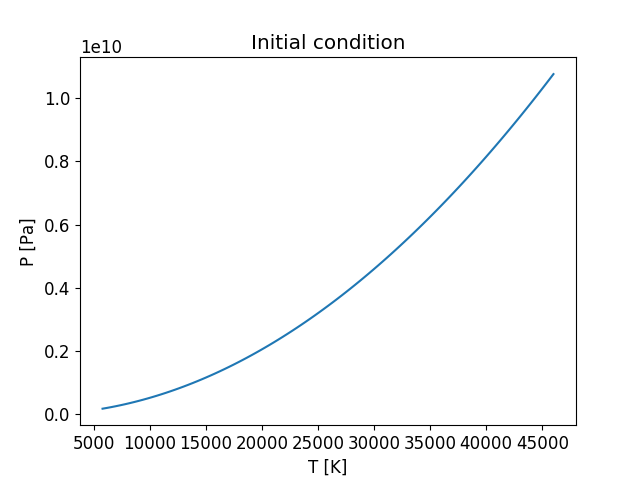
\includegraphics[width = 6cm]{tP_init.png}}
\subfloat[Density.]{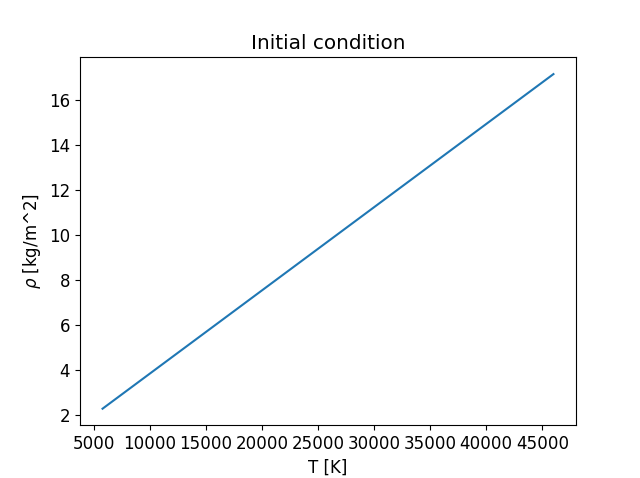
\includegraphics[width = 6cm]{trho_init.png}} \\
\subfloat[Pressure.]{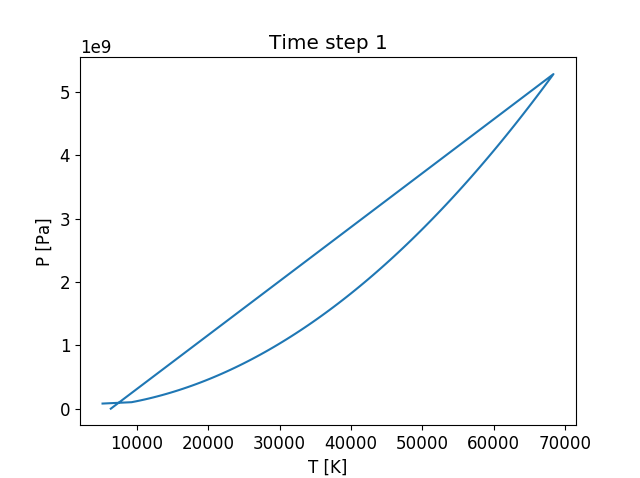
\includegraphics[width = 6cm]{tP_1.png}} 
\subfloat[Density.]{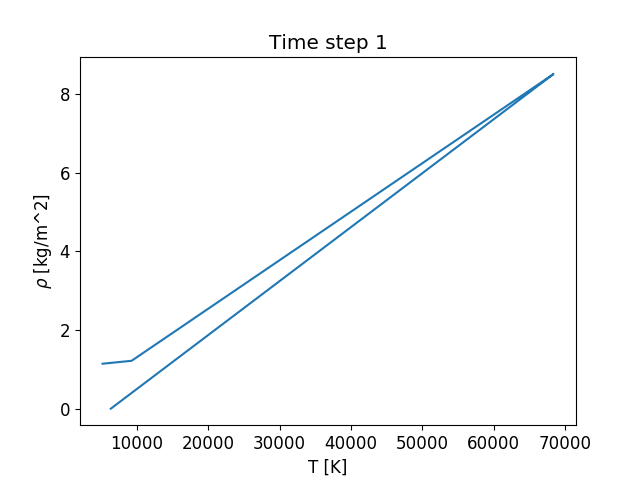
\includegraphics[width = 6cm]{trho_1.png}}
\caption{Figures (a)-(d) shows the y-values pressure and density as a function of temperature for the initial condition ((a) and (b)) and for the first time step ((c) and (d)).}
\label{fig:plot}
\end{figure}
I will here summarize the span of values over the y-values (going from the outside and in) for the initial condition
\begin{itemize}
\item Temperature: 5778 K to 45987 K, steady rise.
\item Pressure: $1.8 \cdot 10^8$ Pa to $1.07 \cdot 10^{10}$ Pa, steady rise.
\item Density: $2.285$ to $17.156$ kg/m$^2$, steady rise.
\end{itemize}

As far as we have gathered, these values are fine, so we consider the initial conditions to have been implemented correctly. Following are span of y-values for the first time step
\begin{itemize}
\item Temperature: $5200$ K to $68378$ K, but last value is $6355$ K.
\item Pressure: $8.1 \cdot 10^7$ to $5.2 \cdot 10^9$ Pa, but last value 0 Pa.
\item Density: $1.14$ to $8.5$ kg/m$^2$, but last value 0.
\item Velocity and momentum: 0 everywhere.
\item Energy: $5.4\cdot 10^7$ to $3.5 \cdot 10^9$, last value 0.
\end{itemize}

As one can see, there are issues with the final values for time steps above 0. The temperature seem to by too high going inwards. The density looks to be too low to begin with.

\section{Problems}
There may be a problem somewhere regarding the pressure gradient in the main calculation loop, as one of the boundary conditions is not used; the pressure gradient at the vertical boundaries $\partial P /\partial y = 0$. I tried updating the density by solving the hydrostatic equation $\partial P/\partial y = -g\rho$ for $\rho$ and calculating the pressure gradient by the central differentiation method. If we calculate the pressure using the gradient for the current time step, we would at $t=0$ cancel the initial condition. We cannot use a pressure gradient to calculate the next time step for the pressure: $P_j^{t+1} = P_j^t + (\partial P/\partial y)dy$.

The particles does not start to move, as the velocities are zero through the simulation (and as a result, the momentum as well). We understand that the particles were supposed to get a velocity from numerical errors in the method we are using, so one can only assume the method used in this paper is faulty. When adding a velocity of 0.001, we found velocities of the same order throughout the simulation.


\section{Comments}
The boundary condition have been checked numerous times, and I very much hope that the error do not lie there. I think I would have gained more from this project had I had a better understanding of the equations, what they do and how they perform. The leap from the previous projects seem a bit steep. I struggle with the idea that the velocities should arise from numerical errors, as I have no control over it.


\begin{thebibliography}{9}

\bibitem{1}
  B. V. Gudiksen,
  \textit{AST3310: Astrophysical plasma and stellar interiors},
  \url{http://www.uio.no/studier/emner/matnat/astro/AST3310/v18/beskjeder/notes_v1.pdf} (downloaded 07.03.18)
\end{thebibliography}






\end{document}
